\let\negmedspace\undefined
\let\negthickspace\undefined
\documentclass[journal]{IEEEtran}
\usepackage[a5paper, margin=10mm, onecolumn]{geometry}
%\usepackage{lmodern} % Ensure lmodern is loaded for pdflatex
\usepackage{tfrupee} % Include tfrupee package

\setlength{\headheight}{1cm} % Set the height of the header box
\setlength{\headsep}{0mm}     % Set the distance between the header box and the top of the text

\usepackage{gvv-book}
\usepackage{gvv}
\usepackage{cite}
\usepackage{amsmath,amssymb,amsfonts,amsthm,mathtools}
\usepackage{algorithmic}
\usepackage{graphicx}
\usepackage{textcomp}
\usepackage{xcolor}
\usepackage{txfonts}
\usepackage{listings}
\usepackage{enumitem}
\usepackage{mathtools}
\usepackage{gensymb}
\usepackage{comment}
\usepackage[breaklinks=true]{hyperref}
\usepackage{tkz-euclide} 
\usepackage{listings}
\def\inputGnumericTable{}                                 
\usepackage[latin1]{inputenc}                                
\usepackage{color}                                            
\usepackage{array}                                            
\usepackage{longtable}                                       
\usepackage{calc}                                             
\usepackage{multirow}                                         
\usepackage{hhline}                                           
\usepackage{ifthen}                                           
\usepackage{lscape}
\begin{document}

\bibliographystyle{IEEEtran}
\vspace{3cm}

\title{3.3.2.25}
\author{EE24BTECH11024 - G. Abhimanyu Koushik
}
% \maketitle
% \newpage
% \bigskip
{\let\newpage\relax\maketitle}

\renewcommand{\thefigure}{\theenumi}
\renewcommand{\thetable}{\theenumi}
\setlength{\intextsep}{10pt} % Space between text and floats

\textbf{Question:}\\
A Triangle $ABC$ can be constructed with side $BC=7cm$, $\angle B=45\degree$, $\angle A=105\degree$. Then construct another triangle whose sides are $\frac{3}{4}$ times the corresponding sides of $\Delta ABC$\\
\textbf{Solution:}
\begin{table}[h!]    
  \centering
  \begin{tabular}[12pt]{ |c|c|c|}
    \hline
    \textbf{Symbol} & \textbf{Value} & \textbf{Description} \\
    \hline
    $\vec{A}$ & \myvec{6\\5} & First point\\
    \hline 
    $\vec{B}$ & \myvec{-4\\3} & Second point\\
    \hline
    $\vec{Y}$ & \myvec{0\\$y$} & Point on Y-Axis equidistant from A and B\\
    \hline
    \end{tabular}

  \caption{Variables Used}
  \label{tab10.5.3.9.1}
\end{table}\\
$\angle C$ can be found as 
\begin{align}
A+B+C&=180\degree\\
105\degree+45\degree+C&=180\degree\\
C&=30\degree
\end{align}
From properties of triangles we get the following equations
\begin{align}
a&=a\\
a&=b\cos(C)+c\cos(B)\\
\frac{b}{\sin(B)}&=\frac{c}{\sin(C)}
\end{align}
Rewriting the equations will give
\begin{align}
a+\brak{0}b+\brak{0}c&=a\\
\brak{0}a+b\cos(C)+c\cos(B)&=a\\
\brak{0}a+b\brak{\sin(C)}+c\brak{-\sin(B)}&=0
\end{align}
It results in the following matrix equation
\begin{align}
  \myvec{1 & 0 & 0\\0 & \cos(C) & \cos(B)\\0 & \sin(C) & -\sin(B)}\times\myvec{a\\b\\c}&=a\myvec{1\\1\\0}
\end{align}
We can find all the side lengths by solving the above matrix equation where $x=\frac{a}{a}$, $y=\frac{b}{a}$, and $z=\frac{c}{a}$.
\begin{align}
  \myvec{1 & 0 & 0\\0 & \frac{\sqrt{3}}{2} & \frac{1}{\sqrt{2}}\\0 & \frac{1}{2} & -\frac{1}{\sqrt{2}}}\times\myvec{x\\y\\z}&=\myvec{1\\1\\0}\\
\end{align}
The augmented matrix for this will be
\begin{align}
  \myvec{1 & 0 & 0 & 1\\0 & \frac{\sqrt{3}}{2} & \frac{1}{\sqrt{2}} & 1\\0 & \frac{1}{2} & -\frac{1}{\sqrt{2}} & 0} \xleftrightarrow[]{R_2 \leftarrow \frac{2}{\sqrt{3}}R_2}\myvec{1 & 0 & 0 & 1\\0 & 1 & \frac{\sqrt{2}}{\sqrt{3}} & \frac{2}{\sqrt{3}}\\0 & \frac{1}{2} & -\frac{1}{\sqrt{2}} & 0}\\
  \xleftrightarrow[]{R_3 \leftarrow 2R_3}\myvec{1 & 0 & 0 & 1\\0 & 1 & \frac{\sqrt{2}}{\sqrt{3}} & \frac{2}{\sqrt{3}}\\0 & 1 & -\sqrt{2} & 0}\\
  \xleftrightarrow[]{R_3 \leftarrow R_2-R_3}\myvec{1 & 0 & 0 & 1\\0 & 1 & \frac{\sqrt{2}}{\sqrt{3}} & \frac{2}{\sqrt{3}}\\0 & 0 & \frac{\sqrt{2}+\sqrt{6}}{\sqrt{3}} & \frac{2}{\sqrt{3}}}\\
  \xleftrightarrow[]{R_3 \leftarrow \brak{\frac{\sqrt{3}}{\sqrt{2}+\sqrt{6}}}R_3}\myvec{1 & 0 & 0 & 1\\0 & 1 & \frac{\sqrt{2}}{\sqrt{3}} & \frac{2}{\sqrt{3}}\\0 & 0 & 1 & \frac{\sqrt{2}}{1+\sqrt{3}}}\\
  \xleftrightarrow[]{R_2 \leftarrow R_2-\brak{\frac{\sqrt{2}}{\sqrt{3}}}R_3}\myvec{1 & 0 & 0 & 1\\0 & 1 & 0 & \frac{2}{1+\sqrt{3}}\\0 & 0 & 1 & \frac{\sqrt{2}}{1+\sqrt{3}}}
\end{align}
The values of $x$,$y$,$z$ are
\begin{align}
x&=1\\
y&=\frac{2}{1+\sqrt{3}}\\
z&=\frac{\sqrt{2}}{1+\sqrt{3}}
\end{align}
The values of $\frac{a}{a}$,$\frac{b}{a}$ and $\frac{c}{a}$ are
\begin{align}
\frac{a}{a}&=1\\
\frac{b}{a}&=\frac{2}{1+\sqrt{3}}\\
\frac{c}{a}&=\frac{\sqrt{2}}{1+\sqrt{3}}
\end{align}
The lengths of sides of first triangle are
\begin{align}
a&=7\\
b&=\frac{14}{1+\sqrt{3}}\\
c&=\frac{7\sqrt{2}}{1+\sqrt{3}}
\end{align}
The lengths of sides of second triangle are
\begin{align}
a_0&=21/4\\
b_0&=\frac{21}{2\brak{1+\sqrt{3}}}\\
c_0&=\frac{21\sqrt{2}}{4\brak{1+\sqrt{3}}}
\end{align}
\begin{figure}[h!]
   \centering
   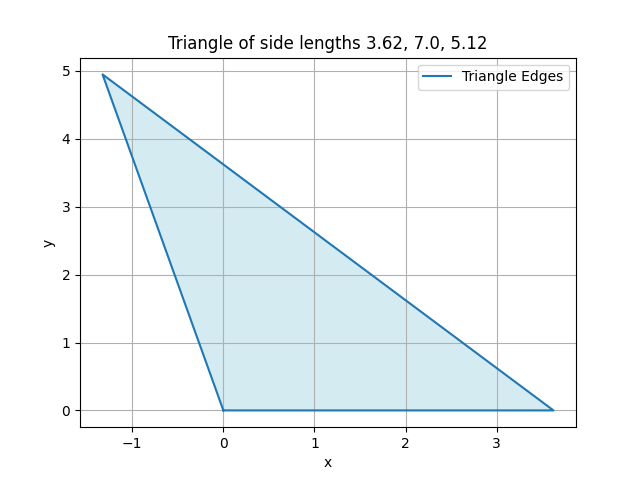
\includegraphics[width=0.7\linewidth]{figs/fig1.png}
   \caption{Triangle with $\angle B=45\degree$, $\angle A=105\degree$ and $BC$ = $7cm$}
\end{figure}
\begin{figure}[h!]
   \centering
   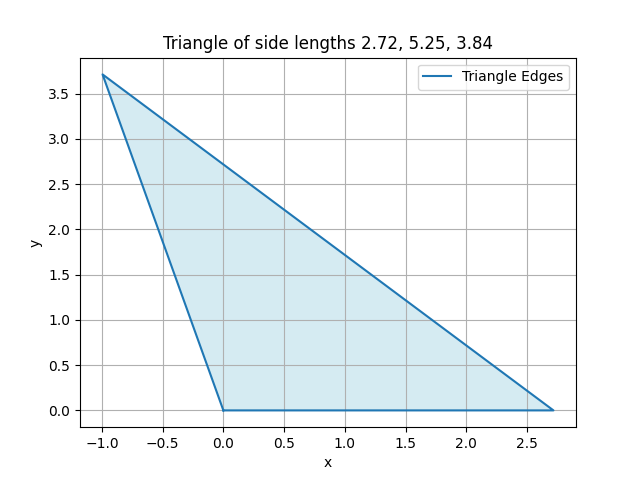
\includegraphics[width=0.7\linewidth]{figs/fig2.png}
   \caption{Triangle with $\angle B=45\degree$, $\angle A=105\degree$ and $BC$ = $7\times\brak{\frac{3}{4}}cm$}
\end{figure}
\end{document}
